
%(BEGIN_QUESTION)
% Copyright 2008, Tony R. Kuphaldt, released under the Creative Commons Attribution License (v 1.0)
% This means you may do almost anything with this work of mine, so long as you give me proper credit

Small relays often come packaged in clear, rectangular, plastic cases.  These so-called ``ice cube'' relays have either eight or eleven pins protruding from the bottom, allowing them to be plugged into a special socket for connection with wires in a circuit.  Note the labels near terminals on the relay socket, showing the locations of the coil terminals and contact terminals:

$$\includegraphics[width=15.5cm]{i03206x01.eps}$$

Draw the necessary connecting wires between terminals in this circuit, so that actuating the normally-open pushbutton switch sends power from the battery to the coil to energize the relay:

\vskip 20pt

$$\includegraphics[width=15.5cm]{i03206x02.eps}$$

\vfil 

This question is typical of those in the ``Pictorial Circuit Diagrams'' worksheet found in the {\it Socratic Instrumentation} practice worksheet collection, except that all answers are provided for those questions.  Feel free to use this practice worksheet to supplement your studies on this very important topic.

\underbar{file i03206}
\eject
%(END_QUESTION)





%(BEGIN_ANSWER)

This is a graded question -- no answers or hints given!
 
%(END_ANSWER)





%(BEGIN_NOTES)

This is by no means the only solution, but it works:

$$\includegraphics[width=15.5cm]{i03206x03.eps}$$

``Ice cube'' style relays are very common in industry, and it is important that students understand how to interpret the pin diagrams on the cases in order to use them in new circuits and to troubleshoot relay circuits that are already built.

%INDEX% Pictorial circuit review (relay circuit)

%(END_NOTES)


